\documentclass{standalone}

%----------------------------------------------------------------------------------------------%
%                                 Packages and basic declarations
%----------------------------------------------------------------------------------------------%

\usepackage[utf8]{inputenc}
\usepackage{pgfplots}
\usepackage{tikz}


%----------------------------------------------------------------------------------------------%
%----------------------------------------------------------------------------------------------%
%                                            DOCUMENT STARTS
%----------------------------------------------------------------------------------------------%
%----------------------------------------------------------------------------------------------%

\begin{document}


%Tikz picture starts%

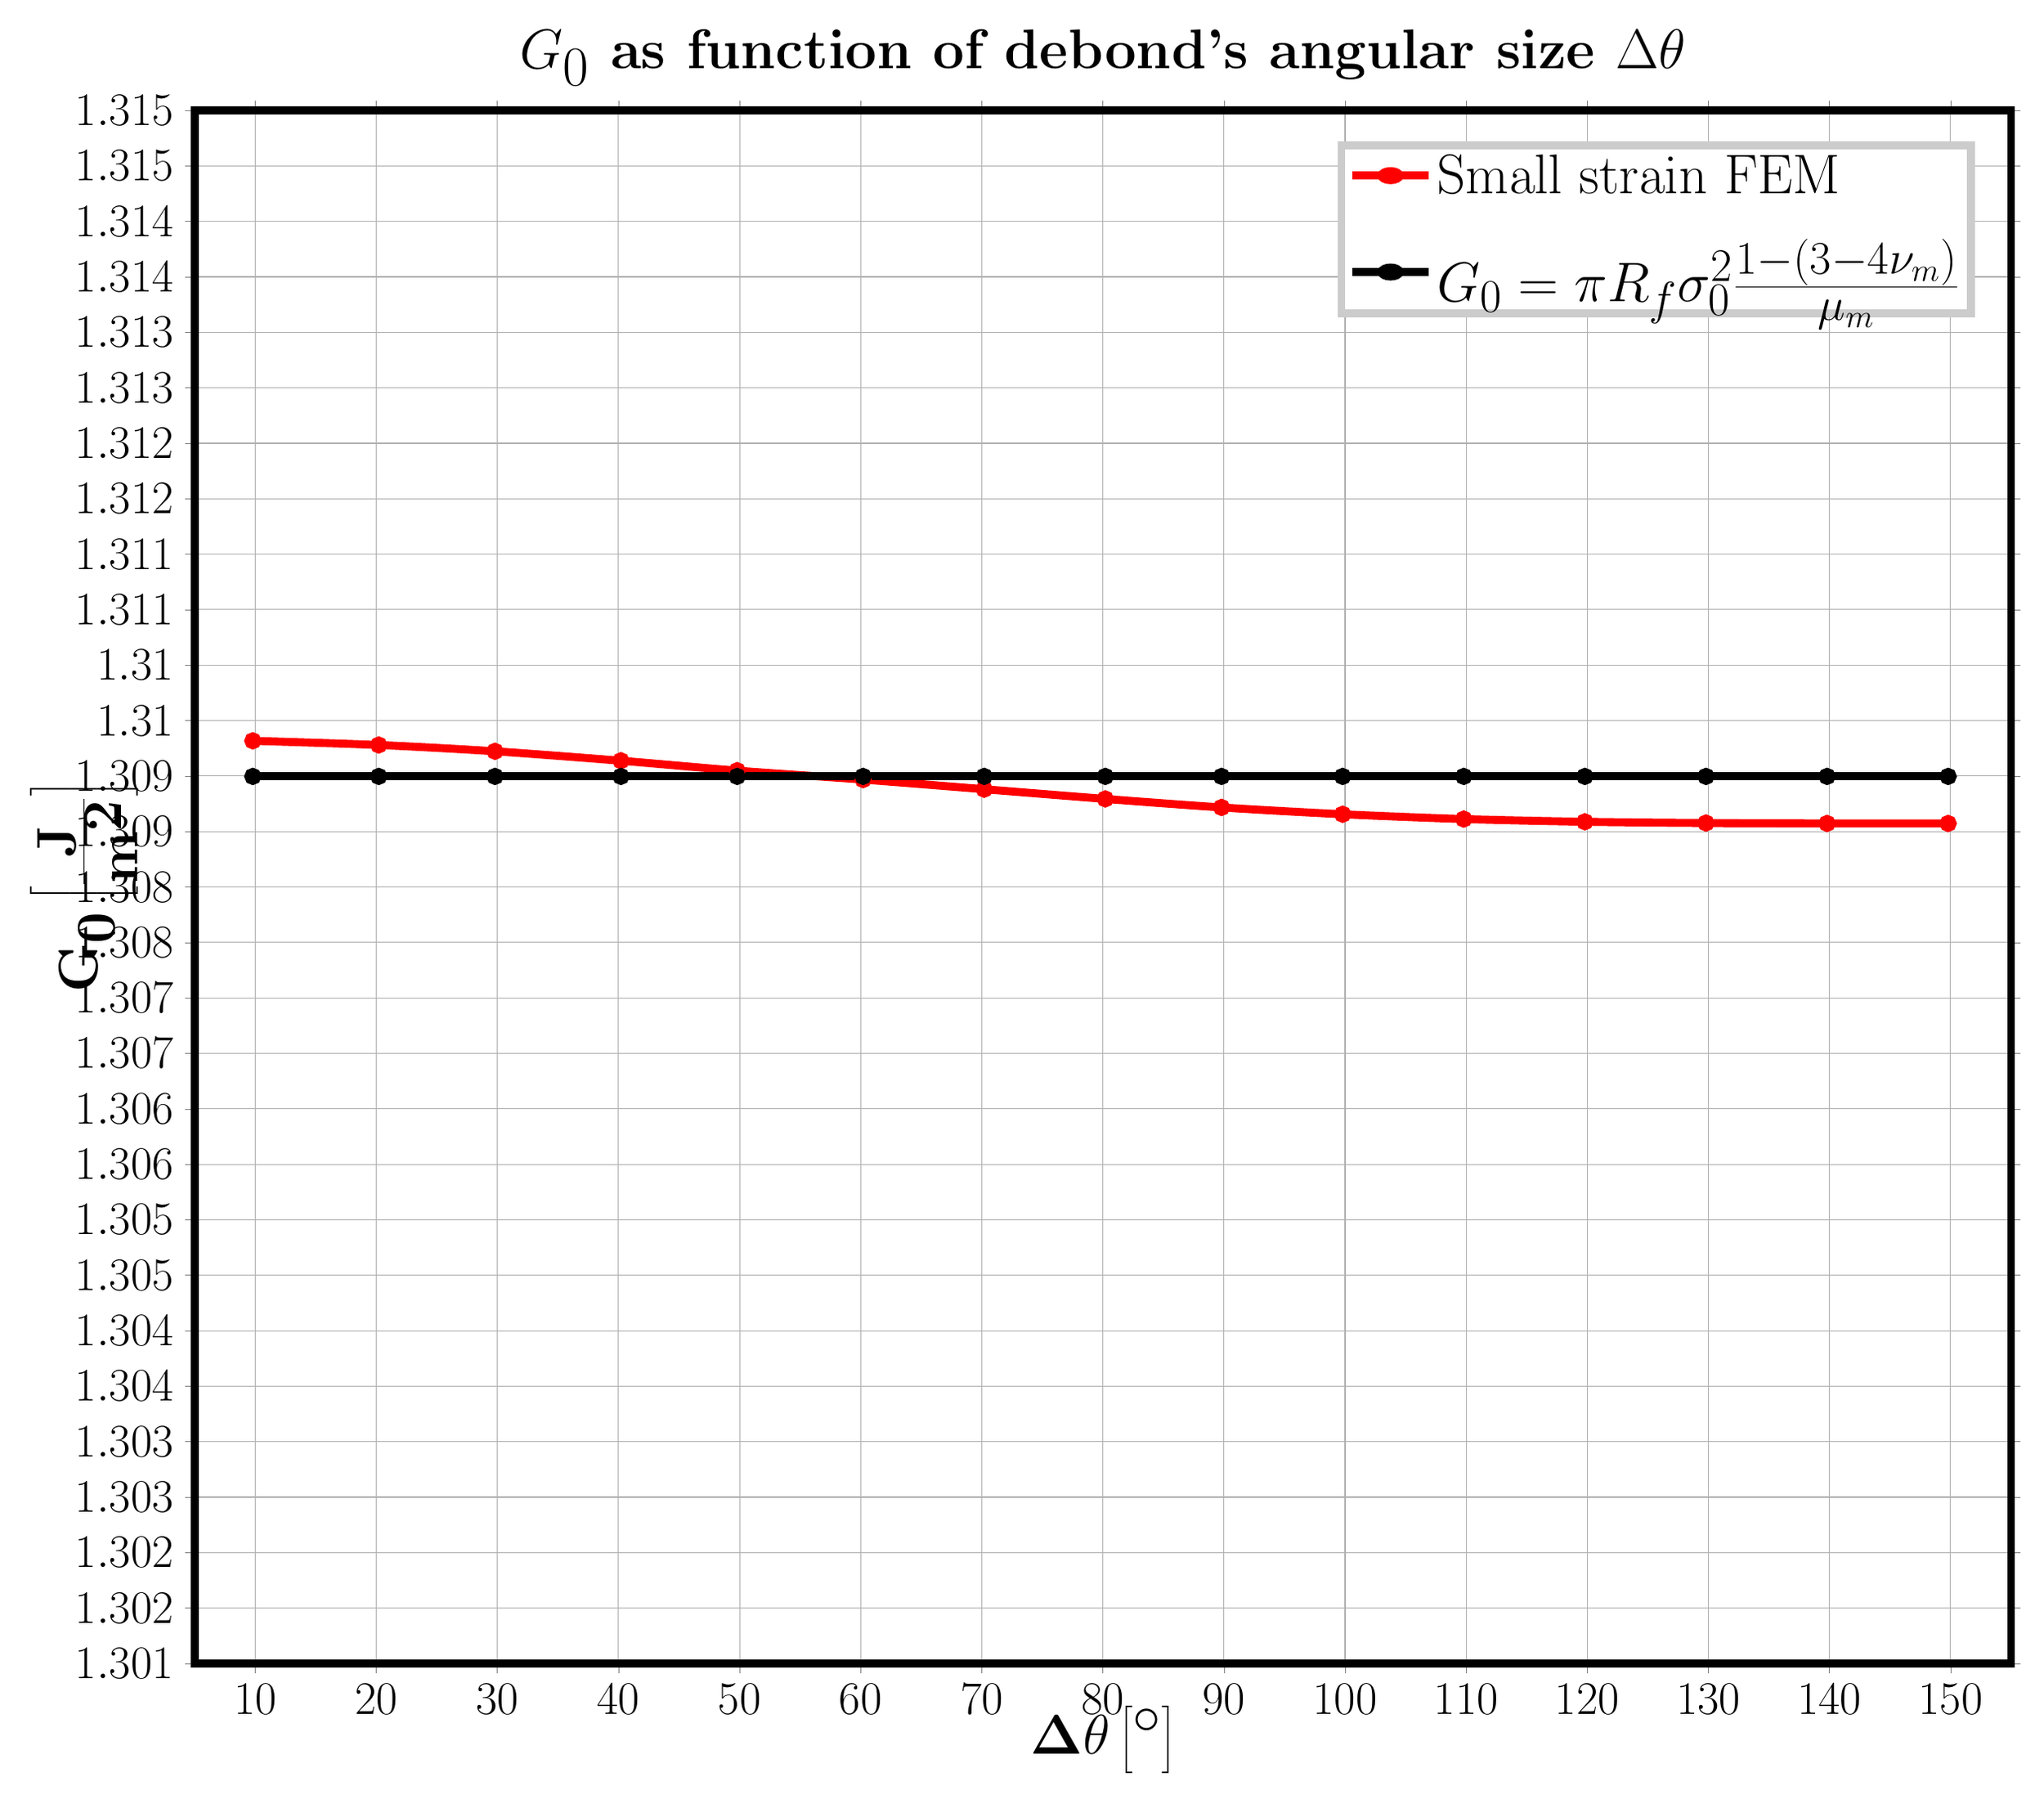
\begin{tikzpicture}

%Tikz axis starts%

\begin{axis}[width=30cm,
title={\bf{$G_{0}$ as function of debond's angular size $\Delta\theta$}},
title style={font=\fontsize{40}{8}\selectfont},
xlabel style={at={(axis description cs:0.5,-0.02)},anchor=north,font=\fontsize{56}{40}\selectfont},
ylabel style={at={(axis description cs:-0.025,.5)},anchor=south,font=\fontsize{48}{40}\selectfont},
xlabel={$\mathbf{\Delta\theta\left[^{\circ}\right]}$},ylabel={$\mathbf{G_{0}\left[\frac{J}{m^{2}}\right]}$},
xmin=5.0,
xmax=155.0,
ymin=1.301,
ymax=1.315,
tick align=outside,
tick label style={font=\huge},
y tick label style={/pgf/number format/precision=3},
xtick={0.0,10.0,20.0,30.0,40.0,50.0,60.0,70.0,80.0,90.0,100.0,110.0,120.0,130.0,140.0,150.0,160.0,170.0,180.0},
xmajorgrids,
x grid style={lightgray!92.026143790849673!black},
ymajorgrids,
y grid style={lightgray!92.026143790849673!black},
line width=1.25mm,
legend style={draw=white!80.0!black,font=\fontsize{28}{24}\selectfont,row sep=15pt},
legend entries={{Small strain FEM},{$G_{0}=\pi R_{f}\sigma_{0}^{2}\frac{1-\left(3-4\nu_{m}\right)}{\mu_{m}}$}},
legend image post style={xscale=2},
legend cell align={left}
]

\addplot[red,smooth,mark=*]
table{
9.8000083551 1.30931795172
20.2001564043 1.30928013341
29.7996713865 1.30922335766
40.1999526243 1.30913821066
49.8000464651 1.30904893443
60.2003242878 1.3089684653
70.1998714969 1.30888165364
80.1999924418 1.30879434432
89.799994075 1.30871754285
99.8000057369 1.30865617419
109.800126682 1.3086129553
119.799673891 1.30858828585
129.800136345 1.3085771285
139.800052385 1.30857328303
149.799859141 1.30857312874
};

\addplot[black,smooth,mark=*]
table{
9.8000083551 1.308996939
20.2001564043 1.308996939
29.7996713865 1.308996939
40.1999526243 1.308996939
49.8000464651 1.308996939
60.2003242878 1.308996939
70.1998714969 1.308996939
80.1999924418 1.308996939
89.799994075 1.308996939
99.8000057369 1.308996939
109.800126682 1.308996939
119.799673891 1.308996939
129.800136345 1.308996939
139.800052385 1.308996939
149.799859141 1.308996939
};

\end{axis}
%Tikz axis ends%


\end{tikzpicture}
%Tikz picture ends%


\end{document}

%----------------------------------------------------------------------------------------------%
%----------------------------------------------------------------------------------------------%
%                                            DOCUMENT ENDS
%----------------------------------------------------------------------------------------------%
%----------------------------------------------------------------------------------------------%
